% !TEX TS-program = pdflatex
% !TEX encoding = UTF-8 Unicode

\documentclass[10pt]{article} % use larger type; default would be 10pt

\usepackage[utf8]{inputenc} % set input encoding (not needed with XeLaTeX)

\usepackage{siunitx}
\usepackage{hyperref}

%%% Examples of Article customizations
% These packages are optional, depending whether you want the features they provide.
% See the LaTeX Companion or other references for full information.

%%% PAGE DIMENSIONS
\usepackage{geometry} % to change the page dimensions
\geometry{a4paper} % or letterpaper (US) or a5paper or....
\geometry{margin=2cm} % for example, change the margins to 2 inches all round
% \geometry{landscape} % set up the page for landscape
%   read geometry.pdf for detailed page layout information

\usepackage{graphicx} % support the \includegraphics command and options
\graphicspath{ {../diagrams/} }

% \usepackage[parfill]{parskip} % Activate to begin paragraphs with an empty line rather than an indent

%%% PACKAGES
\usepackage{booktabs} % for much better looking tables
\usepackage{array} % for better arrays (eg matrices) in maths
\usepackage{paralist} % very flexible & customisable lists (eg. enumerate/itemize, etc.)
\usepackage{verbatim} % adds environment for commenting out blocks of text & for better verbatim
\usepackage{subfig} % make it possible to include more than one captioned figure/table in a single float
% These packages are all incorporated in the memoir class to one degree or another...

%%% HEADERS & FOOTERS
\usepackage{fancyhdr} % This should be set AFTER setting up the page geometry
\usepackage{t1enc}
\usepackage[hungarian]{babel}
\pagestyle{fancy} % options: empty , plain , fancy
\renewcommand{\headrulewidth}{0pt} % customise the layout...
\lhead{}\chead{}\rhead{}
\lfoot{}\cfoot{\thepage}\rfoot{}

%%% SECTION TITLE APPEARANCE
\usepackage{sectsty}
\allsectionsfont{\sffamily\mdseries\upshape} % (See the fntguide.pdf for font help)
% (This matches ConTeXt defaults)

%%% ToC (table of contents) APPEARANCE
\usepackage[nottoc,notlof,notlot]{tocbibind} % Put the bibliography in the ToC
\usepackage[titles,subfigure]{tocloft} % Alter the style of the Table of Contents
\renewcommand{\cftsecfont}{\rmfamily\mdseries\upshape}
\renewcommand{\cftsecpagefont}{\rmfamily\mdseries\upshape} % No bold!

%%% END Article customizations

\title{Programozható LED-fűzéren alapuló reklámpanel - LED füzér vezérlése, adatok kiírása}
\author{Patka Zsolt-András | Számítástechnika BSc}
\date{2019.10.12}

\begin{document}
\maketitle

\section{Beveztő}

A projekt fő célja egy LED-fűzér vezérlése és ennek segítségével egy reklámszöveg megjelenítése. Ehhez egy FPGA lap és egy Worldsemi WS2813 ledfűzér lesz felhasználva.

\section{Követelmények}

\begin{itemize}
\item Protokoll helyes használata
\item Adatok kiírása lehetséges a LED fűzérre
\item Opcionális: 
\begin{itemize}
	\item Pár betű kódolása (3-4)
	\item Betük tárolása BRAM memóriában
\end{itemize}	
\end{itemize}

\section{Állapotok}

Állapotok:
\begin{itemize}
\item READY
	\begin{itemize}
	\item Alap állapot 
	\item "reset" jel esetén ide kerül vissza az automata
	\end{itemize}
\item INIT
	\begin{itemize}
	\item minden LED-et kikapcsol (0x000000-t ír)
	\item "clear" jel esetén ide kerül az automata
	\end{itemize}
\item RENDER
	\begin{itemize}
	\item egyenként küldi a szín információt a LED-ekre
	\item annyiszor végződik el itt a művelet, ahány LED-ünk van
	\item "stop" jel esetén megáll a kiírás
	\end{itemize}
\item DISPLAY
	\item megtörtént a kiírás
\end{itemize}

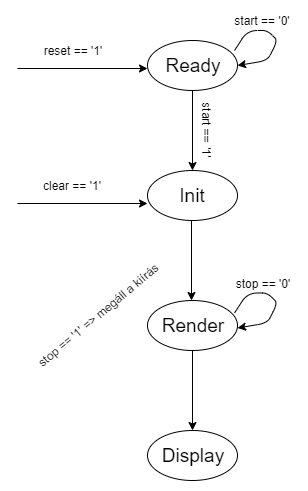
\includegraphics[scale=0.5]{allapotdiagram.png}

\section{Modulok}

\begin{itemize}
\item Következő állapot regiszter \textbf{\textit{Next State Register}}
\item Állapot regiszter \textbf{\textit{State Register}}
\item Szín regiszter \textbf{\textit{Colour Register}}
\item Küldési logika regiszter \textbf{\textit{Transmission Logic Register}}
\end{itemize}

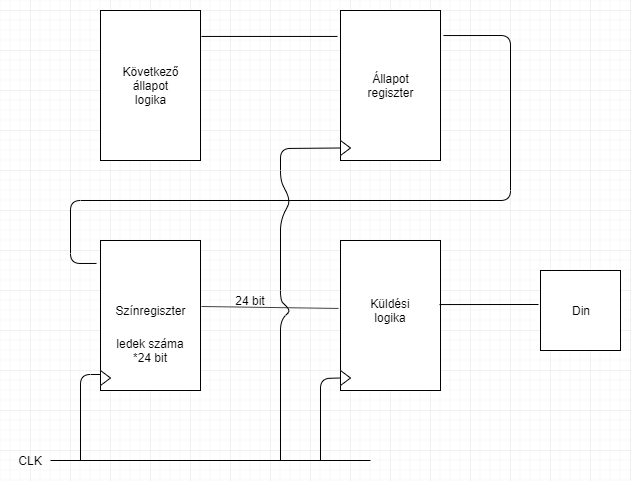
\includegraphics[scale=0.5]{tombvazlat.png}

\subsection{Küldési logika regiszter}

\noindent A küldési logika modul részletesebb lebontása: 

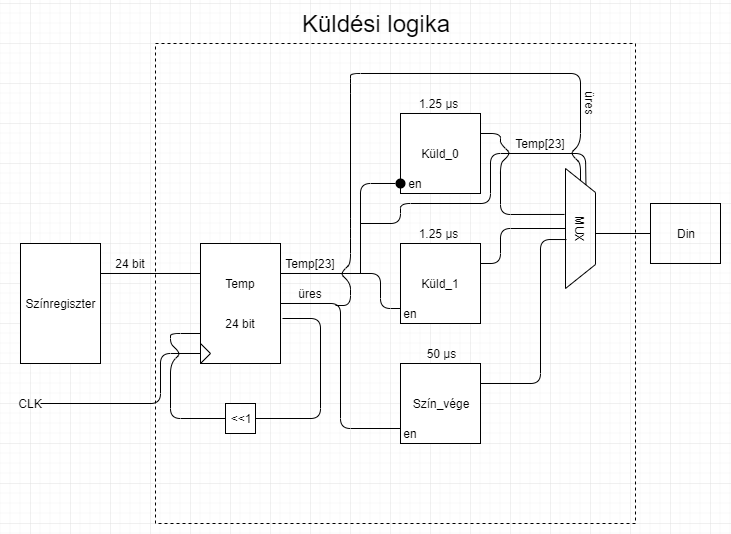
\includegraphics[scale=0.6]{kuldesi_logika.png}


\section{WS2813 egyszálú adatátvitel protokoll leírása}

\indent A LED-eket vezérlő áramkörök egymás után vannak bekötve úgy, hogy az egyik áramkörnek az adatkimenete a következő áramkörnek az adatbemenetét képzi. Egyszálú az adatátvitel, fontos a protokoll betartása, ahhoz, hogy adatokat tudjunk megjeleníteni a LED-fűzéren.

Amikor egy áramkör megkap egy 24 bit-es kódot, akkor ezt addig tárolja amíg más kódot nem kap, vagy a tápforrást el nem veszti.

\subsection{A 24 bit-es kód}

A 24 bit-es kód a következőképpen kell kinézzen:

8 bit GREEN | 8 bit RED | 8 bit BLUE

Az adatátvitel a következő sorrendben kell történjen: 
\begin{enumerate}
	\item GREEN
	\item RED
	\item BLUE
\end{enumerate}

\subsection{Bit-ek küldési sorrendje}

\textbf{Az egyes byte-ok küldését úgy kell elvégezni, hogy az MSB-vel kell kezdeni és haladni az LSB fele.}

\noindent 24 bit-es kód részletesebb felbontása: 
\begin{itemize}
\item \textit{G7 G6 G5 G4 G3 G2 G1 G0 | R7 R6 R5 R4 R3 R2 R1 R0 | B7 B6 B5 B4 B3 B2 B1 B0}
\end{itemize}

\noindent A küldés a következő sorrendben kell elvégződjön: 
\begin{itemize}
\item \textbf{G7 G6 G5 G4 G3 G2 G1 G0 | R7 R6 R5 R4 R3 R2 R1 R0 | B7 B6 B5 B4 B3 B2 B1 B0}
\end{itemize}

\subsection{Időzítések}

Minden 24 bit-es adatátvitel után kell legalább \SI{50}{\micro\second}-ot várakozni. Ez jelzi azt, hogy egy 24 bit-es blokk továbbítása megtörtént.

\noindent Az egyes bit-ek átvitele a következőképp történik:

\begin{itemize}
\item Logikai 1-es
	\begin{itemize}
	\item \SI{0.8}{\micro\second}-ot magas feszűltségen
	\item \SI{0.45}{\micro\second}-ot alacson feszűltségen
	\end{itemize}
\item Logikai 0-ás
	\begin{itemize}
	\item \SI{0.4}{\micro\second}-ot magas feszűltségen
	\item \SI{0.85}{\micro\second}-ot alacson feszűltségen
	\end{itemize}
\item 24 bit-es adatblokk küldése után: 
	\begin{itemize}
		\item $ > \SI{50}{\micro\second}$
	\end{itemize}
\end{itemize}

\noindent A bit-ek továbbításánál egy +/- \SI{150}{\nano\second}-os eltérés megengedett.

A várakozási értékeket nem az adatlapból, hanem az \href{https://learn.adafruit.com/adafruit-neopixel-uberguide}{alábbi} útmutatóból vettem. Az útmutató szerint az adatlapban levő értékek rosszul vannak kiszámolva.

Egyelőre megpróbálok az útmutatóban megadott értékekkel dolgozni. Ha ez nem megfelelő működéshez vezet, akkor veszem az adatlapban levő értékeket.


\end{document}
